\documentclass[Report.tex]{subfiles}

\newcommand{\newaxis}[4]{
\begin{axis}[
    ybar,
    title={#1},
    ymin=#3, ymax=#4,
    bar width=1em,
    legend style={at={(0.5,-0.25)},anchor=north,legend columns=-1},
    enlarge x limits=0.4,
    x tick label style={align=center,text width=1.7cm},
    symbolic x coords={Logistic Regression, Random Forest, Multi-layer Perceptron},
    xtick=data,
    ylabel={#2}
]
}

\begin{document}

\section{Same player identification}

\subsection{Mouse movement features}


\begin{figure}[H]
\newcommand{\plotbar}[2]{
\addplot+[
	discard if not={split}{1},
	discard if not={numSplits}{1},
	discard if not={features}{mouse},
] table [x=model, y=#1,col sep=comma] {data/15-pair-cv.csv};
\addlegendentry{#2}
}
\centering
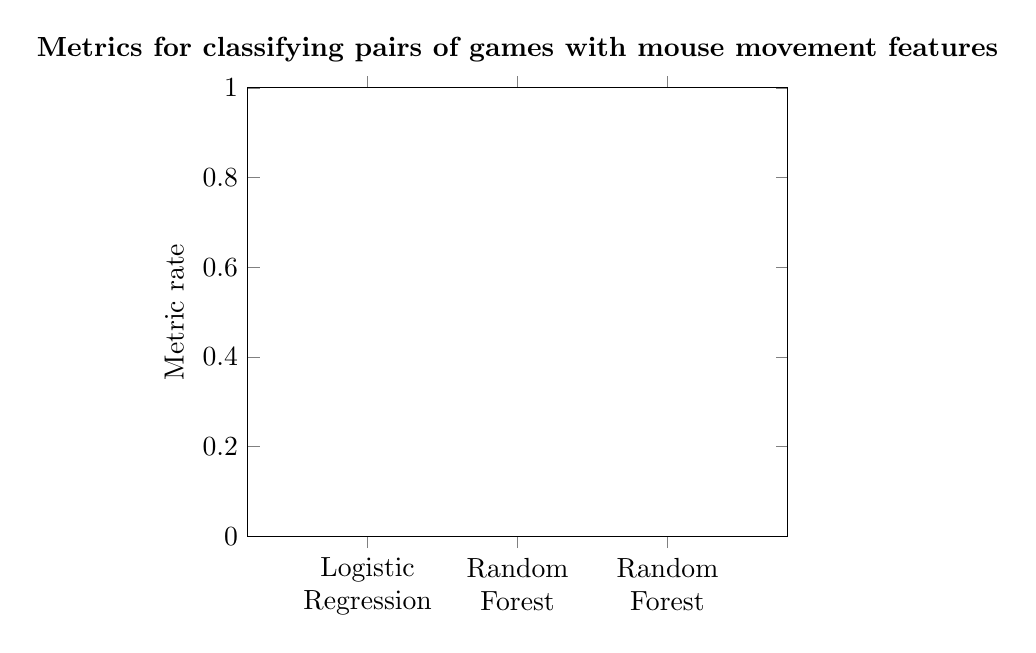
\begin{tikzpicture}
\newaxis{\textbf{Metrics for classifying pairs of games with mouse movement features}}{Metric rate}{0.6}{1.03}

\plotbar{accuracy}{Accuracy}
\plotbar{precision}{Precision}
\plotbar{recall}{Recall}

\end{axis}
\end{tikzpicture}
\end{figure}

\subsection{Game statistic features}

\subsection{Itemisation features}

\subsection{Combined features}
\begin{figure}[H]
\newcommand{\plotbar}[2]{
\addplot+[
	discard if not={split}{1},
	discard if not={numSplits}{1},
	discard if not={features}{#1},
] table [x=model,y=accuracy,col sep=comma] {data/15-pair-cv.csv};
\addlegendentry{#2}
}
\centering
\begin{tikzpicture}
\begin{axis}[
	ybar,
	bar width=1.5em,
	width=11cm,
	legend style={at={(0.5,-0.15)},anchor=north,/tikz/every even column/.append style={column sep=0.5cm}},
	xtick=data,
	enlarge x limits=0.25,
	symbolic x coords={Logistic Regression, Random Forest, Multi-layer Perceptron},
    x tick label style={align=center,text width=2.5cm},
]

\plotbar{mouse}{Mouse movement only}
\plotbar{stats}{Game statistics only}
\plotbar{mouse-stats}{Mouse movement and game statistics}

\end{axis}
\end{tikzpicture}
\caption{Accuracy for pair classification with different features and models.}
\end{figure}


\end{document}

